\documentclass[UTF8]{ctexart}
%%%%%%%%%%%%%%%%%%%%%%%%%%%== 引入宏 ==%%%%%%%%%%%%%%%%%%%%%%%%%%%%%
\usepackage{tikz}
\usetikzlibrary{mindmap,trees}
\usepackage{cite}
\usepackage{framed}
\usepackage{nccbbb}
\usepackage{mathrsfs}
\usepackage{amsthm}
\usepackage{amsmath}	% 使用数学公式
\usepackage{graphicx}	% 插入图片/PDF/EPS 等图像
\usepackage{float}
\usepackage{subfigure}	% 使用子图像或者子表格
\usepackage{geometry}	% 设置页边距
\usepackage{fancyhdr}	% 设置页眉页脚
\usepackage{setspace}	% 设置行间距
\usepackage{hyperref}	% 让生成的文章目录有链接,点击时会自动跳转到该章节
\usepackage{url}
\usepackage{color}
\usepackage{comment}
\usepackage{algorithm}
\usepackage{algorithmic}
\allowdisplaybreaks[1] 
\usepackage{listings}
\usepackage[framed,numbered,autolinebreaks,useliterate]{mcode}
\usepackage{caption2}
 \usepackage{amssymb} 
%\usetikzlibrary{arrows,shapes,chains}
\usepackage{setspace}
\usepackage{comment}
\usepackage{amsfonts}
\usepackage{geometry}
\usepackage{tcolorbox}
\usepackage{titlesec}
\usepackage{titletoc}
\usepackage{setspace}
\geometry{top=12cm,bottom=13cm}
%\usepackage{hyperref}
\usepackage{booktabs}
\renewcommand{\baselinestretch}{1.2}
\setlength{\baselineskip}{20pt}

\usepackage{longtable}

%%%%%%%%%%%%%%%%%%%%%%%%%%== 设置全局环境 ==%%%%%%%%%%%%%%%%%%%%%%%%%%%%
% [geometry] 设置页边距
\geometry{top=2.6cm, bottom=2.6cm, left=2.45cm, right=2.45cm, headsep=0.4cm, foot=1.12cm}
%% 设置行间距为 1.5 倍行距
%\onehalfspacing
%% 设置页眉页脚
%\pagestyle{fancy}
%%\lhead{左头标}
%%\chead{\today}
%%\rhead{152xxxxxxxx}
%%\lhead{文献阅读报告}
%\cfoot{\thepage}
%\rhead{\rightmark}
%\renewcommand{\headrulewidth}{0.4pt}
%\renewcommand{\headwidth}{\textwidth}
%\renewcommand{\footrulewidth}{0pt}

%%%%%%%%%%%%%%%%%%%%%%%%%%== 自定义命令  ==%%%%%%%%%%%%%%%%%%%%%%%%%%%%%%
% 此行使文献引用以上标形式显示
\newcommand{\supercite}[1]{\textsuperscript{\cite{#1}}}
% 此行使section中的图、表、公式编号以A-B的形式显示
\renewcommand{\thetable}{\arabic{subsection}-\arabic{table}}
\renewcommand{\thefigure}{\arabic{subsection}-\arabic{figure}}
\renewcommand{\theequation}{\arabic{subsection}-\arabic{equation}}
% 此行使图注、表注与编号之间的分隔符缺省,默认是冒号:
\renewcommand{\captionlabeldelim}{~}
 \renewcommand{\thefootnote}{}
\renewcommand\tablename{表}
\renewcommand\figurename{图}

\hypersetup{
colorlinks=true,
linkcolor=black,
citecolor=black
}

%===================================== 标题设置  ==========================================
% \heiti \kaishu 为字体设置,ctex 会自动根据操作系统加载字体
\title{\huge{\heiti 文献阅读报告}}
\author{{\kaishu  201928000206036 谢鹏程}\\
{\kaishu  指导教师:\ 袁亚湘\ 院士}\\
{\kaishu xiepengcheng19@mails.ucas.ac.cn}\\
%%\small{\kaishu xiepengcheng19@mails.ucas.ac.cn}\\
{\kaishu 中国科学院计算数学与科学工程计算研究所}\\
{\kaishu 科学与工程计算国家重点实验室}\\
[2pt]
%\small{\kaishu 中国科学院大学数学科学学院201班}\\[2pt]
%\small{Email:}
%\url{csyiji@gmail.com}
}
\date{} % 去除默认日期
%\date{\today}

%===================================== 正文区域  ==========================================

\titlecontents{section}[1cm]{\fontsize{12pt}{\baselineskip}\selectfont}{\hspace*{3em}\contentslabel{2em}\ }%
{}{\titlerule*[0.5pc]{$\cdot$}\contentspage\hspace*{1cm}}%

\titlecontents{subsection}[1cm]{\fontsize{10pt}{\baselineskip}\selectfont}{\hspace*{3em}\contentslabel{2em}\ }%
{}{\titlerule*[0.5pc]{$\cdot$}\contentspage\hspace*{1cm}}%

\renewcommand{\contentsname}{\fontsize{18pt}{\baselineskip}\selectfont \textbf{目\ 录}}



\usepackage{lipsum}

\makeatletter
\newenvironment{breakablealgorithm}
  {% \begin{breakablealgorithm}
   \begin{center}
     \refstepcounter{algorithm}% New algorithm
     \hrule height.8pt depth0pt \kern2pt% \@fs@pre for \@fs@ruled
     \renewcommand{\caption}[2][\relax]{% Make a new \caption
       {\raggedright\textbf{\ALG@name~\thealgorithm} ##2\par}%
       \ifx\relax##1\relax % #1 is \relax
         \addcontentsline{loa}{algorithm}{\protect\numberline{\thealgorithm}##2}%
       \else % #1 is not \relax
         \addcontentsline{loa}{algorithm}{\protect\numberline{\thealgorithm}##1}%
       \fi
       \kern2pt\hrule\kern2pt
     }
  }{% \end{breakablealgorithm}
     \kern2pt\hrule\relax% \@fs@post for \@fs@ruled
   \end{center}
  }
\makeatother


\renewcommand{\large}{\fontsize{13}{14}\selectfont}
\begin{document}

\linespread{1.4}
\large

%%\maketitle
%
%
%
%\begin{figure}[H] %H为当前位置,!htb为忽略美学标准,htbp为浮动图形
%\centering %图片居中
%
\includegraphics[width=0.25\textwidth]{zhongkeyuan.png} %插入图片,[]中设置图片大小,{}中是图片文件名
%%\includegraphics[width=0.9\textwidth]{codes/problem2/BFGS.eps} %插入图  %最终文档中希望显示的图片标题
%
%\label{Fig.main2} %用于文内引用的标签
%\end{figure}
%
%
%
%
%
%
%
%
%
%
%
%%\tableofcontents % 目录内容,注释取消掉可实现目录
%
%
%\newpage
%
%
%\section{\textit{Convex Analysis and Nonlinear Optimization
%: Theory and Examples}阅读报告}
%
%\subsection{整体介绍}
%
%\textit{Convex Analysis and Nonlinear Optimization
%Theory and Examples}一书\cite{borwein2010convex}的作者是数学家Jonathan M. Borwein和Adrian S. Lewis. 首版于2000年,后有再版.
%
%Jonathan M. Borwein于1951年出生于苏格兰圣安德鲁斯一个犹太家庭. 1971年获得西安大略大学的荣誉数学学士,1974年从牛津大学博士毕业. Borwein在1988年和Jonathan Barzilai合作发表文章\textit{Two-Point Step Size Gradient Methods}\cite{barzilai1988two}提出了BB步长. Borwein还是实验数学的杰出公众拥护者. 不幸的是,Borwein于2016年8月仙逝.
%
%Adrian S. Lewis是加拿大英籍数学家,1962年出生于英格兰,1987年获得剑桥大学博士学位 (工程) ,2003年获得Lagrange奖,目前在康奈尔大学从事变分分析和非光滑优化等研究.
%
%两位数学家的伟大情谊也因数学而流芳,在Adrian Stephen Lewis的个人主页上,写有``My longtime friend, mentor, and co-author of Convex Analysis and Nonlinear Optimization, Jon Borwein, passed away in 2016. I miss him."
%
%
%
%\begin{minipage}{0.45\textwidth}
%\centering
%\begin{figure}[H] %H为当前位置,!htb为忽略美学标准,htbp为浮动图形
%\centering %图片居中
%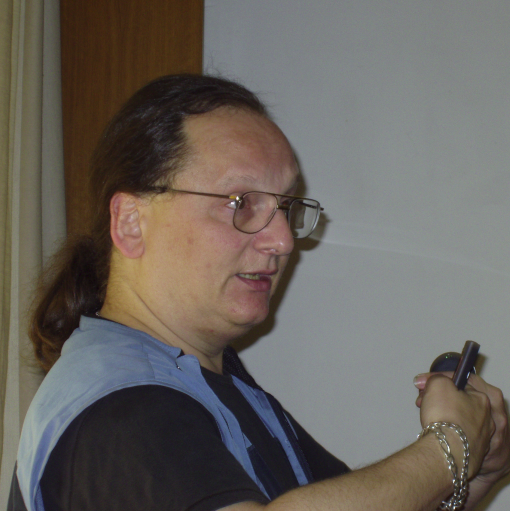
\includegraphics[height=0.7\textwidth]{B.jpg} %插入图片,[]中设置图片大小,{}中是图片文件名
%%\includegraphics[width=0.9\textwidth]{codes/problem2/BFGS.eps} %插入图  %最终文档中希望显示的图片标题
%\caption{Jonathan M. Borwein}
%\label{Jonathan M. Borwein} %用于文内引用的标签
%\end{figure}
%\end{minipage}
%\begin{minipage}{0.45\textwidth}
%\centering
%\begin{figure}[H] %H为当前位置,!htb为忽略美学标准,htbp为浮动图形
%\centering %图片居中
%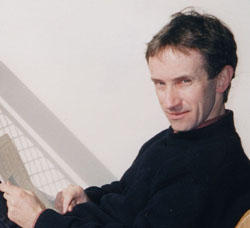
\includegraphics[height=0.7\textwidth]{A.jpg} %插入图片,[]中设置图片大小,{}中是图片文件名
%%\includegraphics[width=0.9\textwidth]{codes/problem2/BFGS.eps} %插入图  %最终文档中希望显示的图片标题
%\caption{Adrian S. Lewis}
%\label{Adrian S. Lewis} %用于文内引用的标签
%\end{figure}
%\end{minipage}
%
%\vspace{0.5cm}
%
%
%
%本书主要介绍凸分析和非线性优化的理论和例子,适用于广大读者. 结合了数学优化和现代分析,主要围绕凸性和对偶性展开.
%
%许多重要的分析问题都有启发性的优化公式,因此可以通过我们的主要变分工具来解决: 次梯度、最优性条件、对偶性、度量正则性等许多方法. 一般而言,凸性思想是从经典分析到现代分析的各个分支过渡的中心: 从线性分析到非线性分析,从光滑到不光滑等. 因此,尽管本书反复使用某些优化模型来说明主要结果 (诸如线性和半定规划对偶性等模型) ,但始终强调抽象模型和符号的功能.
%
%在本书之前已经存在有关有限维凸分析的参考书籍. 自上世纪70年代以来,Rockafellar的经典凸分析教材\cite{rockafellar1970convex}开始普及,最近也出现了更广泛的此类分析教材,本书的目的是要推广其他相关书籍的结果,从而激励更多相关研究.
%
%本书追求简洁而不是系统化,这也是为了避免陷入技术细节的泥潭. 本书的行文风格是相对非正式的: 例如,每个部分的叙述都为结论设置了上下文. 与此同时,本书重视各种独立的方法,希望展示一些令人难忘的定理等,本书在阐述过程中没有讨论算法,而是尽可能给出涉及到的重要参考文献. 此外,本书还介绍了无限维的优化中的问题和挑战. 
%
%\subsection{内容脉络}
%
%本书思路清晰、内容简明扼要且涵盖面广,思路脉络图如图\ref{全书思路概览图}所示. 具体如下:
%
%\newtheorem{zhang}{章目}
%
%\begin{zhang}
%本书的首章介绍了背景知识,包括Euclidean空间、对称矩阵. 
%
%{\small$\bullet$} 在Euclidean空间一节介绍了基本分离定理,并回顾了Bolzano-Weierstrass 定理,同时介绍了全局极小点的存在性.在练习和评注中介绍了凸锥、回收锥、强分离定理、仿射集等基本知识.
%
%{\small$\bullet$} 在对称矩阵一节中引入了矩阵空间的内积$\left<X,Y\right>=tr(XY)$, 并给出了Fan不等式$tr(XY)\le \lambda(X)^T\lambda(Y)$及其特殊情况Hardy-Littlewood-Polya不等式. 同时给出了数值代数中的著名定理Birkhoff定理. 在本节的例子和评注中,进一步地给出了与矩阵相关的具体例子和不等式,如平方根迭代和Fan-Cauchy-Schwarz不等式等.
%
%
%\end{zhang}
%
%\begin{zhang}
%
%本书的第二章围绕不等式约束展开,包括最优性条件、择一性定理和最大方程及一阶条件.
%
%{\small$\bullet$} 在最优性条件一节里,介绍了法锥、必要的和充分的一阶最优性条件、线性约束的一阶条件以及二阶条件等, 在例子和评注中介绍了法锥的一些例子、自对偶锥、仿射集的法锥以及Rayleigh商和割线方程下的BFGS更新公式等.
%
%
%{\small$\bullet$} 在择一性定理一节里,介绍了Gordan定理以及大名鼎鼎的Farkas引理,也即: 
%\newtheorem*{thm}{定理}
%\begin{thm}
%对于点$a^1,a^2,\cdots,a^m$和$\mathbb{E}$中的$c$以下两个系统中有且只有一个系统有解:
%\begin{flalign*} 
%&(1)\ \sum_{i=1}^{m} \mu_{i} a^{i} =c, \quad 0 \leq \mu_{1}, \mu_{2}, \ldots, \mu_{m} \in \mathbb{R}; \\
%&(2)\ \left\langle a^{i}, x\right\rangle \leq 0 , \text {对于} i=1,2, \ldots, m,\langle c, x\rangle>0, x \in \mathbb{E}.&
%\end{flalign*} 
%\end{thm}
%定理的两个系统有且只有一个系统有解这一结果也体现了为什么叫做``择一性定理".
%
%{\small$\bullet$} 在最大函数和一阶条件一节中介绍了最大函数$g(x)=\max\limits_{i=0,1,\cdots,m}\{g_i(x)\}$,$g(x)$的引入考虑了非光滑性(即使$g_0,g_1,\cdots,g_m$均光滑). 紧接着介绍了最大函数的方向导数$g^{\prime}(\bar{x} ; d)=\max _{i \in K}\left\{\left\langle\nabla g_{i}(\bar{x}), d\right\rangle\right\}$. 随后给出了Lagrange函数$L(x ; \lambda)=f(x)+\sum_{i=1}^{m} \lambda_{i} g_{i}(x)$和局部极小点处的Fritz John条件($\lambda_{0} \nabla f(\bar{x})+\sum_{i \in I(\bar{x})} \lambda_{i} \nabla g_{i}(\bar{x})=0$). 以及假设Mangasarian-Fromovitz约束条件 (MFCQ)和Karush-Kuhn-Yucker条件. 并在例子中介绍了KKT的``失败”问题以及H{\"o}lder不等式等.
%
%
%\begin{figure}[H] %H为当前位置,!htb为忽略美学标准,htbp为浮动图形
%\centering %图片居中
%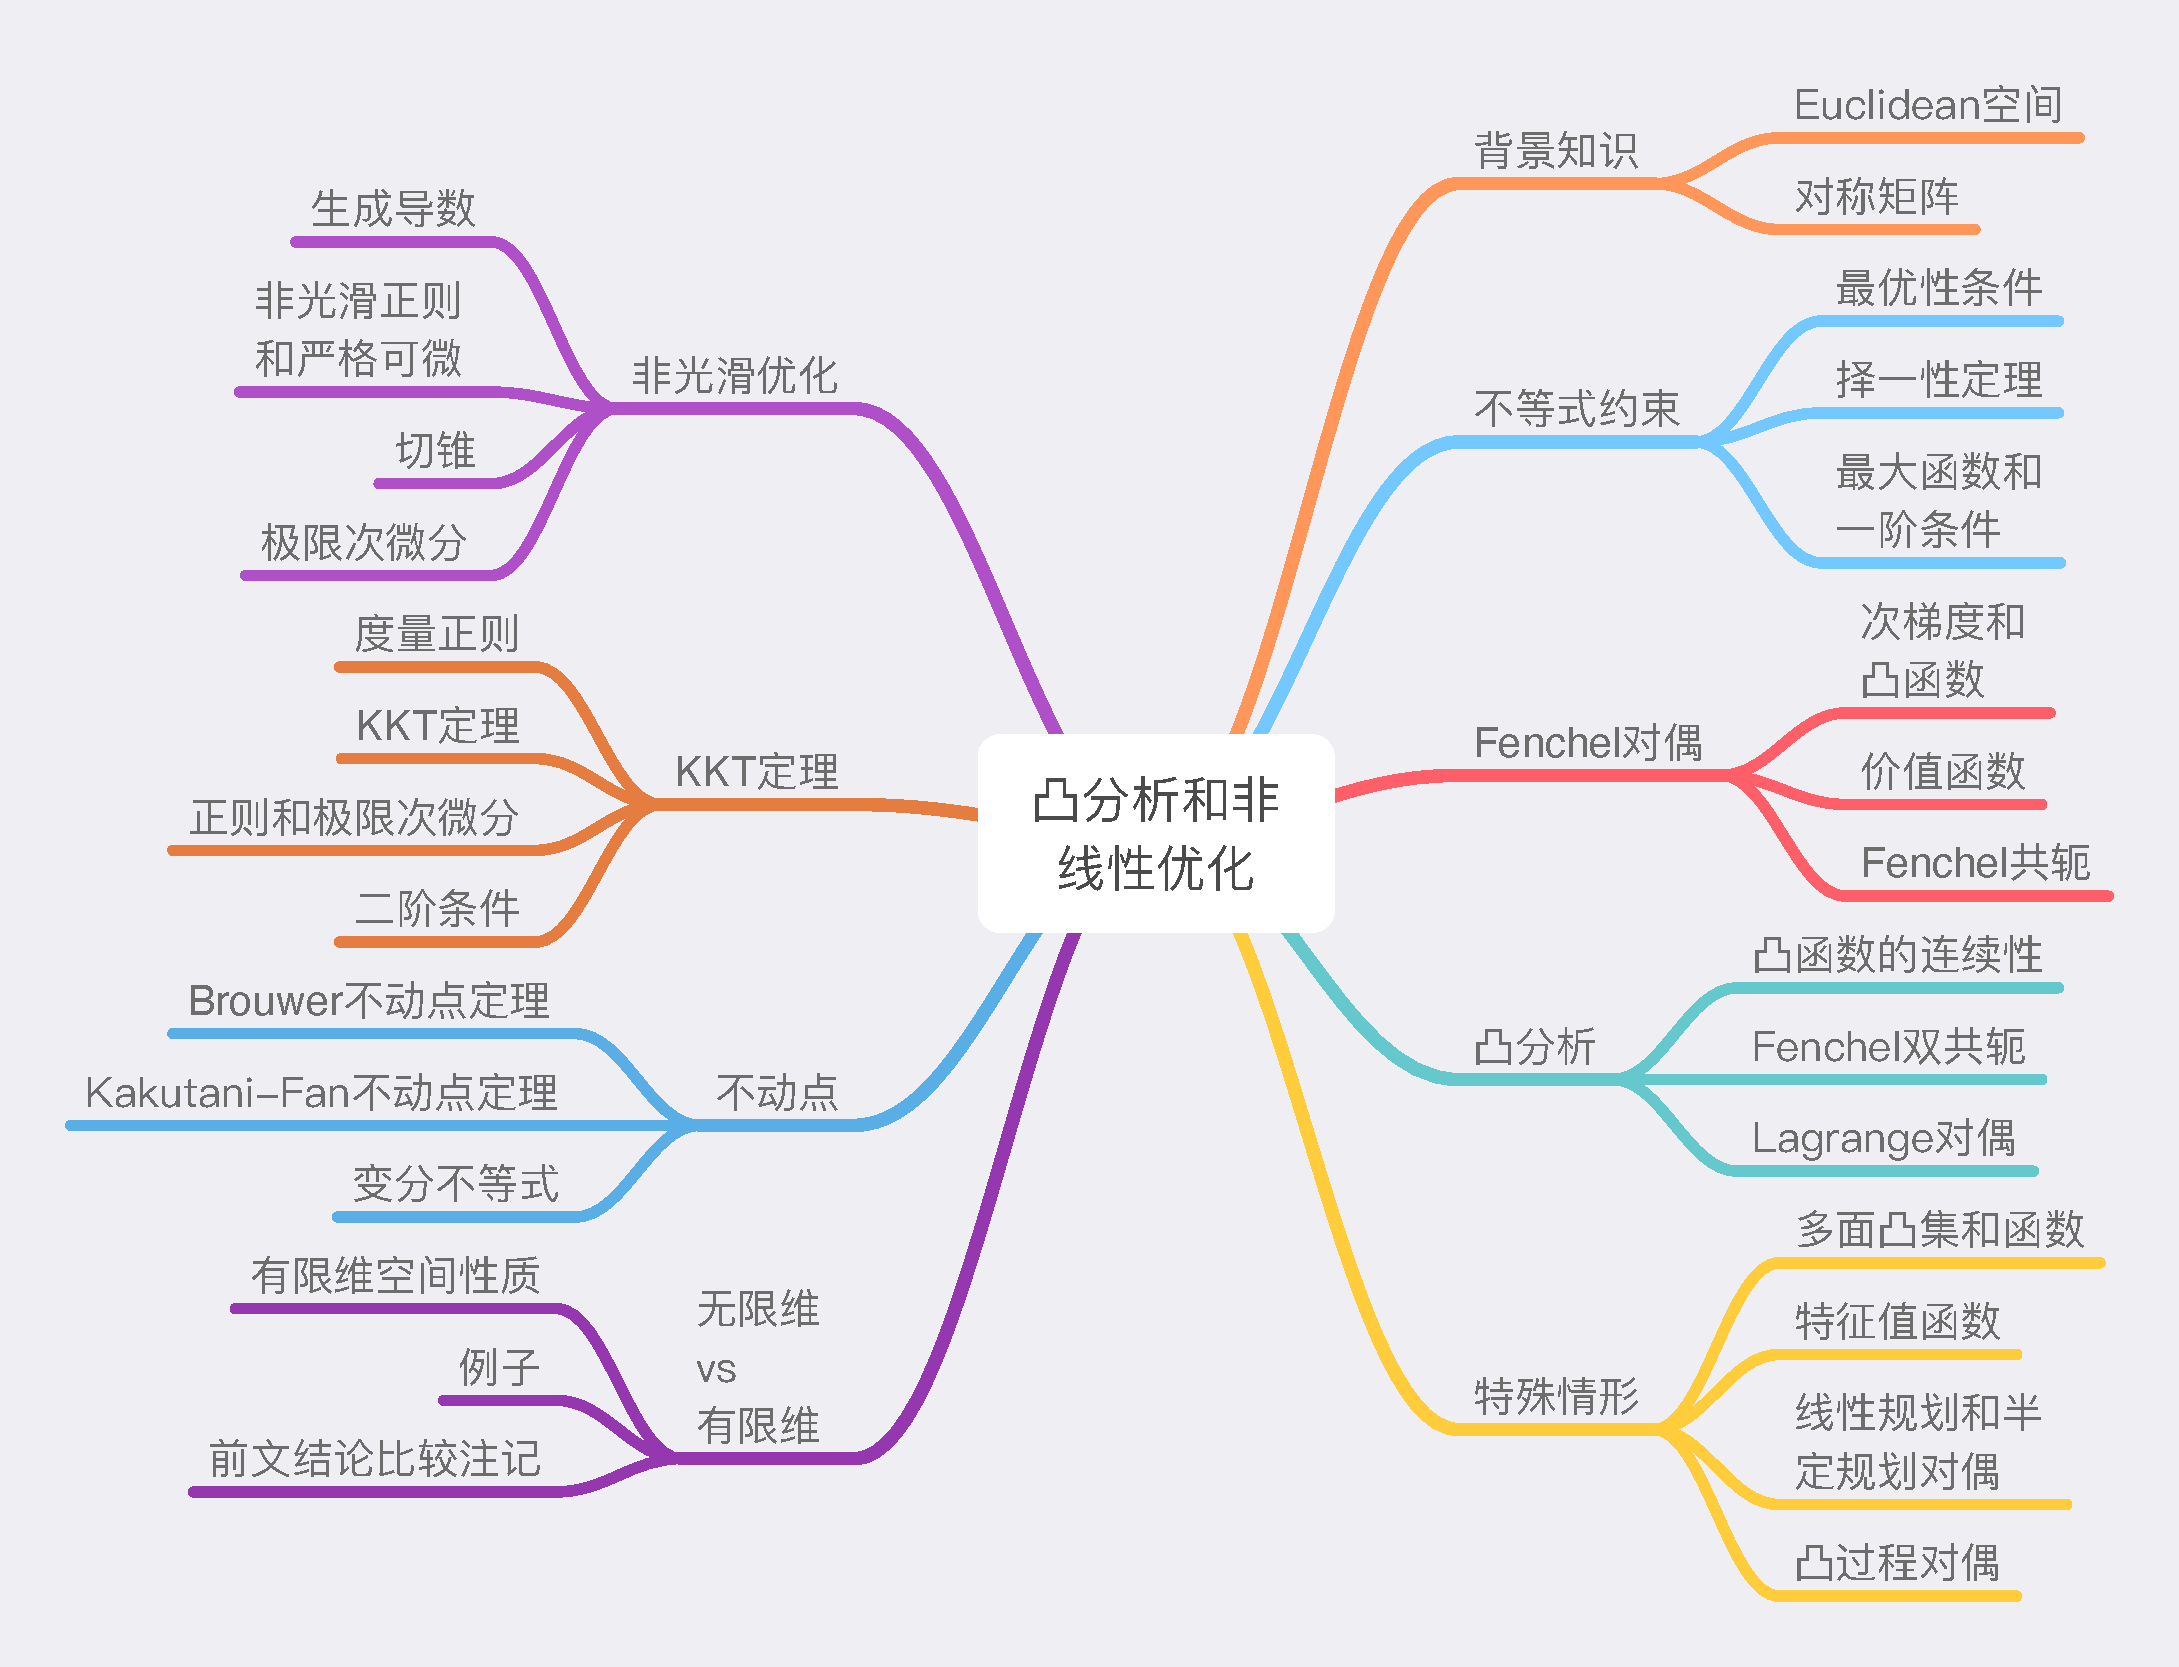
\includegraphics[height=0.75\textwidth]{凸.pdf} %插入图片,[]中设置图片大小,{}中是图片文件名
%%\includegraphics[width=0.9\textwidth]{codes/problem2/BFGS.eps} %插入图  %最终文档中希望显示的图片标题
%\caption{全书思路概览图}
%\label{全书思路概览图}
%\end{figure}
%\end{zhang}
%\begin{zhang}
%本书的第三章主要介绍了Fenchel对偶理论, 包括次梯度和凸函数、价值函数和Fenchel共轭.
%
%{\small$\bullet$} 在次梯度和凸函数一节里,首先引入了次线性的概念以及方向导数的次线性性质. 紧接着给出了次梯度的定义
%$$\partial f(\bar{x})=\{\phi | \langle\phi, x-\bar{x}\rangle \leq f(x)-f(\bar{x}),\mbox{对于$\mathbb{E}$中所有的$x$}\}.
%$$
%然后给出了最优点处的次梯度相关条件,即点$\bar{x}$是极小点当且仅当$0\in \partial f(\bar{x})$成立.
%本章节的重点是用方向导数来局部地描述凸函数的次梯度,鉴于此,本节相继给出了次梯度和方向导数的关系、最大函数公式、凸函数的G{\^a}teaux可微性以及凸性的Hessian矩阵刻画.在例子和评注中,分别给出了次梯度和凸函数的具体例子, 其中也包括log障碍函数.
%
%{\small$\bullet$} 在价值函数一节里,首先给出了Lagrange乘子在互补松弛条件下的理解. 随后基于Lagrange乘子给出了Lagrange充分条件和Lagrange必要条件.
%
%{\small$\bullet$} 
%在第3节中引入和研究Fenchel共轭主要是为了更深入地理解上节所给的凸系统的Lagrange必要条件.对于函数$h:\mathbb{E}\rightarrow[-\infty,+\infty]$,其Fenchel共轭为$h^{*}(\phi)=\sup _{x \in \mathbb{E}}\{\langle\phi, x\rangle-h(x)\}$,随后一并给出了关于矩阵和向量的log障碍函数
%$$\operatorname{lb}(x)=\left\{\begin{array}{ll}-\sum_{i=1}^{n} \log x_{i}, & \text {如果} x \in \mathbf{R}_{++}^{n} \\ +\infty, & \text {否则}\end{array}\right.\ 
%\text{和}\ 
%\operatorname{ld}(X)=\left\{\begin{array}{ll}-\log \operatorname{det} X, & \text {如果} X \in \mathbf{S}_{++}^{n} \\ +\infty, & \text {否则}\end{array}\right.
%$$
%以及共轭$\operatorname{lb}^{*}(x)$和$\operatorname{ld}^{*}(X)$. 
%
%之后给出了Fenchel-Young不等式: $h(x)+h^{*}(\phi) \geq\langle\phi, x\rangle$,等式成立当且仅当$\phi \in \partial h(x)$.
%
%接下来介绍了Fenchel对偶意义下的原始和对偶值
%$$
%\begin{aligned} p &=\inf _{x \in \mathbb{E}}\{f(x)+g(A x)\} \\ d &=\sup _{\phi \in \mathbb{Y}}\left\{-f^{*}\left(A^{*} \phi\right)-g^{*}(-\phi)\right\} \end{aligned}
%$$
%的弱对偶性和法则$\partial(f+g \circ A)(x) \supset \partial f(x)+A^{*} \partial g(A x)$以及等式成立条件,也即$0 \in \operatorname{core}(\operatorname{dom} g-A \operatorname{dom} f)$或$A \operatorname{dom} f \cap \operatorname{cont} g \neq \emptyset$成立.
%
%此外还介绍了线性约束的Fenchel对偶以及自对偶锥、Krein-Rutman极锥法则和双极锥、指向锥等. 本节还通过较多例子对共轭、对偶进行了更细致的展现, 包括$\mathbb{R}$上的凸函数共轭对表.
%
%\end{zhang}
%
%\begin{zhang}
%
%第4章主要是凸分析的内容,包括凸函数的连续性、Fenchel双共轭、Lagrange对偶.
%
%{\small$\bullet$} 在凸函数的连续性一节中,作者先后介绍了局部有界性、凸函数的连续性,还有核和内部、双极集、支撑超平面等概念,以及将紧凸集用极点的凸锥表示的Minkowski定理.
%
%{\small$\bullet$} 在Fenchel双共轭一节,主要关注和其双共轭函数相等的凸函数的相关性质. 在介绍完下半连续的定义 ($\liminf h\left(x^{r}\right)\left(=\lim _{s \rightarrow \infty} \inf _{r \geq s} h\left(x^{r}\right)\right) \geq h(x)$) 后, 相继给出了Fenchel双共轭 (等价性) 定理、支撑函数定理和Moreau-Rockafellar定理等以及严格对偶定理. 上述定理将凸函数和其共轭函数的性质进一步进行了联系. 最后给出了关于$h=h^{**}$时相关性质的回答:
%对于凸函数$h: \mathbb{E} \rightarrow[-\infty,+\infty]$,
%在$h$有限时,对于任一点$x$,$h(x)=h^{**}(x)$当且仅当$h$在点$x$处下半连续.
%
%本节的例子和评注分别介绍了下半连续性和闭性的关系、中点凸性、次梯度的逆、闭次梯度、支撑函数等.
%
%{\small$\bullet$} 第3节主要介绍了Lagrange对偶,我们回到前面所研究过的凸系统
%%$$
%%\left\{\begin{array}{cccc}\inf & f(x) & & \\ \text {使得} & g(x) & \leq & 0 \\ & x & \in & \mathbb{E}.\end{array}\right.
%%$$
%\begin{align*}
%\inf\ &f(x)  \\
%\text {使得}\  &g(x)  \leq  0 \\ 
%& x  \in  \mathbb{E}.
%\end{align*}
%该系统可以写成
%$$
%p=\inf _{x \in \mathbb{E}} \sup _{\lambda \in \mathbb{R}_{+}^{m}} L(x ; \lambda),
%$$
%其中$L(x ; \lambda)=f(x)+\lambda^{T} g(x)$,对应的对偶为: 
%$$
%d=\sup _{\lambda \in \mathbb{R}_{+}^{m}} \inf _{x \in \mathbb{E}} L(x ; \lambda).
%$$
%同时我们借助原始值函数$v(b)=\inf \{f(x) | g(x) \leq b\}$来对Lagrange对偶进行分析,相继给出对偶最优值定理、零对偶间隙定理、对偶达到定理、原始达到定理等. 在例子和评注中给出了松弛性、紧性,以及对偶的相关例子和Duffin对偶间隙、信赖域子问题对偶间隙等.
%
%\end{zhang}
%
%\begin{zhang}
%
%第5章主要介绍特殊情形,包括多面体凸集和函数、特征值函数、线性规划和半定规划的对偶、凸过程对偶.
%
%{\small$\bullet$} 多面体凸集和函数一节首先在前面所介绍的多面体和其对应的多面函数基础上定义了有限生成多面体和有限生成函数,并给出了关于多面函数和有限生成函数的两个主要结果. 并得到一个集合或函数是多面的当且仅当其是有限生成的重要结果,此后为了展示很多线性代数算子是保多面性的,给出了多面代数定理和多面Fenchel对偶以及混合Fenchel对偶.
%
%在例子和评注中,介绍了多面体的切锥、生成Fenchel对偶、几何规划等.
%
%{\small$\bullet$} 特征值函数一节中给出了和Fenchel相关的一些经典矩阵分析中的特征值不等式. 在用$\delta_{\mathbb{S}^n_+}=\delta_{\mathbb{R}^n_+}\circ\lambda$和$\operatorname{ld}=\operatorname{lb}\circ\lambda$将向量和矩阵关联并给出对称函数的定义($f(x)=f([x])$)之后,给出了对称函数的谱共轭定理($(f \circ \lambda)^{*}=f^{*} \circ \lambda$)、Davis结论(可以用于证明函数的凸性和闭性),并利用共轭公式和Fenchel-Young不等式给出谱的次梯度以及可微性的相关结论.
%
%在本节的例子和评注中还给出了凸谱函数的6个例子.
%
%{\small$\bullet$} 第3节主要介绍了线性规划和半定规划的对偶,线性规划为
%\begin{align*}
%\inf\ \  &\langle c, x\rangle \\ 
%\text {使得}\ \ &\left\langle a^{i}, x\right\rangle-b_{i} \leq  0, \text {对于} i=1,2, \ldots, m \\
% &x \in \mathbb{R}^{n},
%\end{align*}
%此外,如下的矩阵优化问题称为半定规划
%\begin{align*}
%\inf\ \  &\text{tr}(CX) \\ 
%\text {使得}\ \ &\text{tr}(A_{i}X)=b_{i}, \text {对于} i=1,2, \ldots, m \\
% &X \in \mathbb{S}^{n}_+.
%\end{align*}
%值得注意的是,将矩阵空间的内积定义为$\langle A,B\rangle:=\text{tr}(AB)$则可以有效地对以上两种情况进行统一. 本节主要介绍了锥规划对偶、线性规划对偶和半定规划对偶. 例子和评注中还提到了线性规划和半定规划的中心路.
%
%{\small$\bullet$} 在凸过程对偶一节中,介绍了多值函数和过程, 然后介绍了多值函数的开性和下半连续性.紧接着介绍了关于凸过程的一系列结论,包括联合过程对偶定理、范数对偶定理、开映射定理、闭图像定理等.
%
%\end{zhang}
%
%\begin{zhang}
%
%第6章主要介绍非光滑优化,包括生成导数、非光滑正则和严格可微、切锥以及极限次微分.
%   
%{\small$\bullet$} 前面介绍了凸函数及其次梯度,对于非凸函数,仅有次梯度作为分析工具已不够用,类比凸函数的方向导数,第6章第1节针对在点$x$处Lipschtiz连续的实函数给出了生成导数的定义: 
%\begin{flalign*}
%&\text{Dini生成导数: }\ f^{-}(x ; h)=\liminf _{t_{1}\downarrow0} \frac{f(x+t h)-f(x)}{t},\\
%&\text{Clarke生成导数: }\ f^{\circ}(x ; h)=\limsup _{y \rightarrow x, t\downarrow 0} \frac{f(y+t h)-f(y)}{t}=\inf _{\delta>0}\sup_{\|y-x\| \leq \delta, \atop 0<t<\delta} \frac{f(y+t h)-f(y)}{t},\\
%&\text{Michel-Penot生成导数: }f^{\diamond}(x ; h)=\sup _{u \in \mathbb{E}} \limsup _{t\downarrow 0} \frac{f(x+t h+t u)-f(x+t u)}{t}.&
%\end{flalign*}
%并指出关系$f^{-}(x ; \cdot) \leq f^{\diamond}(x ; \cdot) \leq f^{\circ}(x ; \cdot) \leq K\|\cdot\|$,
%以及非光滑最大公式定理$\partial_{-} f(x) \subset \partial_{\diamond} f(x) \subset \partial_{\circ} f(x) \subset K B$和
%\begin{align*}
%&f^{\circ}(x ; h)=\max \left\{\langle\phi, h\rangle | \phi \in \partial_{\circ} f(x)\right\}\\
%&f^{\diamond}(x ; h)=\max \left\{\langle\phi, h\rangle | \phi \in \partial_{\diamond} f(x)\right\}
%\end{align*}
%以及Clarke次梯度的非光滑法则(Michel-Penot次梯度类似)
%\begin{align*}
%&\partial_{\mathrm{o}}(f+g)(x) \subset \partial_{\mathrm{o}} f(x)+\partial_{\mathrm{o}} g(x),\\
%&\partial_{\mathrm{o}}(f \vee g)(x) \subset \operatorname{conv}\left(\partial_{\mathrm{o}} f(x) \cup \partial_{\mathrm{o}} g(x)\right).
%\end{align*}
%最后给出了非光滑函数的最优性必要条件.
%
%{\small$\bullet$} 前文对于约束优化的最优性必要条件给出了两个形式不同的结果: 一者是G{\^a}teaux可微的Karush-Kuhn-Tucker条件,二者是基于凸性的Lagrange必要性条件. 非光滑正则和严格可微一节尝试对两个形式进行统一.先后给出了唯一Michel-Penot次梯度定理、凸函数正则性定理、严格可微的定义和定理、唯一Clarke次梯度定理和Clarke次梯度定理: 当函数$f$在点$x$处局部Lipschitz,且$S\subset \mathbb{E}$测度为0时,函数$f$在点$x$处的Clarke次梯度为$\partial_{\circ} f(x)=\operatorname{conv}\left\{\lim _{x} \nabla f\left(x^{r}\right) | x^{r} \rightarrow x, x^{r} \notin S\right\}$.
%
%{\small$\bullet$} 考虑到我们通常将约束优化问题$\inf \{f(x) | x \in S\}$转化为$f+\delta_{S}$,而指示函数$\delta_S$并不一定是局部Lipschitz的,因此切锥一节介绍了到集合$S$的距离函数$d_{S}(x)=\inf \{\|y-x\| | y \in S\}$.紧接着介绍了精确罚函数 ($f+Ld_S$) 定理、Clarke切锥: $T_{S}(x)=\left\{h | d_{S}^{\circ}(x ; h)=0\right\}$、Dini方向导数引出的锥$K_{S}(x)=\left\{h | d_{S}^{-}(x ; h)=0\right\}$,以及切锥定理、凸切锥定理、Clarke法锥定理 ($N_{S}(x)=T_{S}(x)^{-}$,$\operatorname{cl}\left(\mathbf{R}_{+} \partial_{\circ} d_{S}(x)\right)$) ,并得到了我们所关注的非光滑必要性条件($0 \in \partial_{\diamond} f(x)+N_{S}(x)$)和Contingent必要性条件($-\nabla f(x) \in K_{S}(x)^{-}$).
%
%{\small$\bullet$} 第4节主要介绍极限次梯度,我们已经观察到,次梯度越小,基于其得到的最优性必要条件越强.但是Dini次梯度过于小,很可能不满足求和法则,$\partial_{-}(f+g)(x) \notin \partial_{-} f(x)+\partial_{-} g(x)$. 鉴于此,本节介绍了极限次梯度
%$$
%\partial_{a} f(x)=\left\{\lim _{r} \phi^{r} | x^{r} \rightarrow x, \phi^{r} \in \partial_{-} f\left(x^{r}\right)\right\},
%$$
%这样就可以使得Dini的图像成为闭的.并由此得到结论
%$$
%\partial_{a} f(x)=\bigcap_{\delta>0} \operatorname{cl}\left(\partial_{-} f(U(f, x, \delta))\right),
%$$
%其中$U(f, x, \delta)=\{z \in \mathbb{E}|\|z-x\|<\delta,| f(z)-f(x) |<\delta\}$. 此外,本节还介绍了模糊和法则并最终给出极限次梯度求和法则.
%
%
%\end{zhang}
%
%\begin{zhang}
%
%第7章主要围绕Karush-Kuhn-Tucker定理展开,包括度量正则性、Karush-Kuhn-Tucker定理、极限次微分以及二阶条件.
%
%{\small$\bullet$} 第1节引入度量正则化,在本书前面部分主要的优化模型是不等式约束,本节针对等式约束问题$\inf \{f(x) | h(x)=0\}$,使用contingent锥来线性化其可行域$h^{-1}(0)$. 在得到$K_{h^{-1}(h(x))}(x) \subset N(\nabla h(x))$的结论后又相继给出Ekeland变分原则和函数$h$在$S$上的点$x$处弱度量正则的定义: $d_{S \cap h^{-1}(h(x))}(z) \leq k\|h(z)-h(x)\|$(对于所有离$x$近的$S$中的点$z$). 最后给出了满射和度量正则定理以及本节的主要结论Liusternik定理: 如果$h$在点$x$处严格可微,则集合$h^{-1}(h(x))$在$x$处切正则,且$K_{h^{-1}(h(x))}(x)=N(\nabla h(x))$.
%
%在本节的例子和评注中介绍了Lipschitz扩张、闭性和Ekeland原则等.
%
%
%{\small$\bullet$} 第2节介绍了Karush-Kuhn-Tucker定理,为了得到问题$\inf \{f(x) | x \in S\}$在局部最优点处的最优性必要条件,本节大致分三步进行分析:
%
% 1.扩展Liusternik定理,以描述contingent锥$K_S(\bar{x})$;
%
%  2.使用Farkars引理来计算锥的极锥;
%
%   3. 应用contingent必要条件得到最终结果. 
%
%   接着介绍了后面需要的Mangasarian-Fromovitz约束条件(MFCQ),即: 积极约束函数$g_i$在$\bar{x}$处Frechet可微,等式约束映射$h$在$\bar{x}$处严格可微,且 $\{p \in N(\nabla h(\bar{x})) |\langle\nabla g_{i}(\bar{x}), p\rangle<0 \text {对于} i \in I(\bar{x})\}$ 非空.
%
%在MFCQ成立下,又给出了可行域$S$的contingent锥:$$K_{S}(\bar{x})=\left\{p \in N(\nabla h(\bar{x})) |\left\langle\nabla g_{i}(\bar{x}), p\right\rangle \leq 0 \text { for } i \text { in } I(\bar{x})\right\}.$$
%并最终得到MFCQ下的Karush-Kuhn-Tucker条件
%$$
%\nabla f(\bar{x})+\sum_{i \in I(\bar{x})} \lambda_{i} \nabla g_{i}(\bar{x})+\nabla h(\bar{x})^{*} \mu=0.
%$$
%例子和评述部分也围绕具体约束进行了举例.
%
%
%{\small$\bullet$} 第3节主要介绍度量正则和极限次梯度,前面介绍了弱度量正则,这里更进一步地给出了度量正则$d_{S \cap h^{-1}(y)}(z) \leq k\|h(z)-y\|$. 并得到了极限次梯度和正则性定理: 对于点$x\in S$,如果没有非零元满足条件$0 \in \partial_{a}\langle w, h(\cdot)\rangle(x)+N_{S}^{a}(x)$,则$h$在$S$上$x$处度量正则. 紧接着在此基础上继续给出了满射和度量正则定理,以及到水平集的距离的相关定理.
%
%{\small$\bullet$} 第4节主要介绍了二阶条件,首先介绍了二次Frechet可微,即
%$\left(\nabla^{2} h(\bar{x}) v\right)(v)=\nabla^{2} h(\bar{x})(v, v)$,且知其二次模型为$h(\bar{x}+v)=h(\bar{x})+\nabla h(\bar{x}) v+\frac{1}{2} \nabla^{2} h(\bar{x})(v, v)+o\left(\|v\|^{2}\right)$.之后再给出了二阶最优性必要条件和充分条件.
%
%\end{zhang}
%
%\begin{zhang}
%
%
%第8章主要围绕不动点展开,包括Brouwer不动点定理、Kakutani-Fan不动点定理以及变分不等式.
%
%{\small$\bullet$} 第1节介绍Brouwer不动点定理,之所以考虑不动点问题,是因为多数优化中的问题可以简化为求解非线性方程组$h(x)=0$, 而这与不动点问题$f(x)=x$ (其中$f=I-h$) 是等价的.
%
%大多数不动点存在性定理分为三类: 
%
%1.基于Banach收缩原理的几何结果; 
%
%2.序假设结果; 
%
%3.拓扑结果.
%
%首先给出收缩的定义: 称$f$是一个收缩,如果$\|f(x)-f(y)\| \leq \gamma_{f}\|x-y\|$对于所有$x, y \in C$成立,其中$\gamma_{f}<1$. 然后给出了Banach收缩定理: 任意$\mathbb{E}$的闭子集上的收缩有唯一不动点. 
%
%对于不是收缩的映射,本节给出了更为基本的Brouwer定理: 任意$\mathbb{E}$的非空紧凸子集上的连续自映射有不动点.
%
%在给出Brouwer定理的证明之前,本节相继给出了Stone-Weierstrass定理、变量改变定理和关键的拓扑结果收缩定理.
%
%{\small$\bullet$} 第2节进一步介绍关于不动点理论的结果以及Kakutani-Fan不动点定理. 前面的Brouwer不动点定理集中研究从非空凸集映到自身的函数, 在本节我们扩展到研究多值函数$\Omega$到自身的不动点(满足$x\in\Omega(x)$),围绕此,先后给出了极大单调定理、Kakutani-Fan定理 (本节的核心结论,将Brouwer定理拓展到了多值函数情形) 、紧性的一般定义、整体分割定理、Cellina定理(近似挑选定理,引入了多值函数的连续挑选,即满足$f(x)\in\Omega(x)$的所有连续映射$f$),并通过构造满足$d_{G(\Omega)}\left(x, f_{r}(x)\right)<\frac{1}{r}$的连续自映射$f_r$给出了Kakutani-Fan定理的证明. 若将多值函数的条件由USC换为LSC,可以得到本节最后给出的Michael定理(和前面的Cellina结论平行).
%
%{\small$\bullet$} 本书前文围绕变分不等式$\left\langle\nabla f\left(x_{0}\right), x-x_{0}\right\rangle \geq 0$展开,该不等式是凸集上的可微函数$f$在局部极小点的最优性必要条件,如果$f$仅是凸函数,该关系为$0 \in \partial f\left(x_{0}\right)+N_{C}\left(x_{0}\right)$(非光滑也有类似结果). 第3节主要是使用不动点理论来研究多值函数的变分不等式, 简单的说,就是寻找$C$中的点$x_0$使得$0 \in \Omega\left(x_{0}\right)+N_{C}\left(x_{0}\right)$,可以转化为寻找$(I-\Omega) \circ P_{C}: \mathbb{E} \rightarrow \mathbb{E}$的不动点的问题. 变分不等式的可解性定理保证了该问题解的存在性.该定理本质上和Kakutani-Fan不动点定理等价. 此外,又介绍了非紧集合下的变分不等式,并介绍了作为非紧集合例子的多值互补问题以及属于该类问题的线性规划问题和变分不等式的关系.
%
%在例子和评注中,介绍了包含cuscos的变分不等式、单调互补问题、Fan最小最大不等式以及半定互补性等.
%
%
%\end{zhang}
%
%\begin{zhang}
%
%
%第9章是关于无限维和有限维的补充说明,也对前文所介绍的结论分章节在无限维空间条件下进行了注记和比较总结.
%
%{\small$\bullet$} 本章主要是简要体现前面几章所得到的结论对有限维的依赖,我们的不少主要结论可以直接扩展到自反的Banach空间,但是有些性质不能直接拓展到无限维,这主要是因为凸集的紧性和支撑性是关键保障. 本节提前列出了相关的定义, 如$f$在$x$处的$\beta$-导数等.
%
%{\small$\bullet$} 第2节主要介绍了3组有限维空间的等价性定理. 
%第1组定理是关于有限维空间和其闭性、函数的连续性和单位闭球的紧性.
%第2组定理围绕G{\^a}teaux可微性和相关超平面展开.
%第3组定理涉及到弱$*$收敛、依范数收敛以及次微分的有界性等.
%
%{\small$\bullet$} 第3节主要列举了同上节定理相关的部分有限维、无限维空间
%例子,如吸收集$X=\cup\{t C | t \geq 0\}$、唯一次梯度、范数函数、支撑点、闭锥的和、Banach空间中的多面体、$l_p$上分离函数的半连续性、子空间的和.
%
%{\small$\bullet$} 第4节针对前面8章的结论在无限维空间和有限维空间进行分析比较.
%
%关于第1章,无限维空间中的分离定理即是Hahn-Banach定理的几何版本,是泛函分析的基本. 此外,无限维空间中的Bolzano-Weierstrass定理在空间满足一定条件后成立.
%
%关于第2章中所介绍的不等式约束问题的分析,最优性一阶必要性条件在一般的空间下成立,但是只有在Hilbert空间的闭凸集或在严格凸范数的弱紧凸集这一限制下有最近点的存在性和唯一性.
%
%关于第3章中所介绍的Fenchel对偶,主要的结果如Fenchel对偶性、
%Lagrange乘子定理等在一般设置下均仍然成立.
%
%关于一般线性空间的凸性,在无限维空间,因为可能存在有界闭凸集没有支撑超平面的情况,故Minkowski定理在一些假设下成立,其中的一个Minkowski的延拓版本是Banach空间的任一弱紧凸子集是它的强暴露点的闭凸锥. 此外,开映射定理和Moreau-Rockafellar定理均在一般空间下成立,而且和Fenchel对偶等价的Lagrange对偶也可以在一般情况下相应的建立.
%
%无限维空间的线性算子理论较为完善,Banach代数的谱理论和紧算子以及特征值的相关结果均有相应的研究,闭凸过程也是线性映射的自然拓展.
%
%关于第6章的非光滑优化,在无限维空间,虽然Hadamard和Frechet导数不再相等, 相应的计算法则和均值定理等可以拓展.  
%
%关于第7章KKT定理所介绍的变分原理等,在无限维情况下可以得到拓展,只要把握住变分的核心: 在函数的几乎极小点处考察其是否为函数受到轻微扰动后的极小点. 相应地,约束条件在无限维空间的情况中也有不同的形式.   
%
%第8章的不动点理论中的Banach收缩以及Brouwer定理等均可以得到良好的拓展.
%
%\end{zhang}
%
%\begin{zhang}
%
%第10章列出了正文和例子与评注中涉及到的主要结果及其出处.
%
%\end{zhang}
%
%
%\subsection{例子选摘}
%本书配有不少例子和评注,大都是有所出处的经典例子,值得深究,
%此处简单给出相关的部分证明,更全面的证明可参看书中所给参考文献.
%
%\newtheorem{ques}{摘例}
%
%
%\begin{ques}
%
%\textbf{凸约束优化的最优性必要条件: }
%
%设 $f: \mathbb{E}\rightarrow\mathbb{R}$连续可微,且$C\subseteq\mathbb{E}$是闭凸集,$L>0$. 则下面两命题等价.
%
%(i) $\langle \nabla f (\bar{x}), x-\bar{x}\rangle\geqslant  0,\forall x\in C$.
%
%(ii) $P_C(\bar{x}-\frac{1}{L}\nabla f(\bar{x}))=\bar{x}$.
%
%
%%\newtheorem{proof}{证明}[section]
%\begin{proof}
%
%\noindent \\
%(i) $\Rightarrow$(ii):  根据(i), 我们知道 
%$$\langle \bar{x}-\frac{1}{L}\nabla f(\bar{x})-\bar{x},x-\bar{x}\rangle=-\frac{1}{L}\langle\nabla f(\bar{x}),x-\bar{x}\rangle\leqslant  0,\forall x\in C.$$
%此外, 我们知道$C\subseteq\mathbb{E}$是闭凸集, 因此我们可以由投影定理得到
%$P_{C}(\bar{x}-\frac{1}{L}\nabla f(\bar{x}))=\bar{x}$.
%
%
%\noindent 
%(ii)$\Rightarrow$(i):  如果$P_{C}(\bar{x}-\frac{1}{L}\nabla f(\bar{x}))=\bar{x}$成立, 我们可以得到$\langle \bar{x}-\frac{1}{L}\nabla f(\bar{x})-\bar{x},x-\bar{x}\rangle\leqslant  0, \forall x\in C$, 因此$\langle\frac{1}{L}{\nabla f(\bar{x})}, x-\bar{x}\rangle\geqslant  0,$ 故$\langle\nabla f(\bar{x}),x-\bar{x}\rangle\geqslant  0$ 对于所有的$x\in C$成立. 
%
%由上我们证明了上面的命题是等价的.
%%%%%%%%%%%%%%%%%%%%%
%
%
%\end{proof}
%
%\end{ques}
%
%\begin{ques}
%
%\textbf{闭锥的切锥: }
%
%设$K\subseteq  \mathbb{E}$是一个闭锥. 则
%
%(a) $T_{k}(0)=K$.
%
%(b) $\mathbb{R}_+\{\bar{x}\}\subseteq  T_{k}(\bar{x})$ $\forall\bar{x}\in K$.
%
%
%
%\begin{proof}
%
%\noindent \\
%\textbf{(a)}
%\textbf{ (i)}$ K\subseteq  T_{k}(0)$:
%
%对于任意的$\bar{x}\in K$, 我们知道$\frac{1}{k}\bar{x}\in K,\  k\in\mathbb{N}$, 这是因为$K$是一个闭锥. 令$t_k=\frac{1}{k}\rightarrow 0$,且$x_{k}=t_{k}\bar{x}=\frac{1}{k}\bar{x}$. 因此$\mathop{lim}\limits_{k\rightarrow\infty}\frac{x_{k}-0}{t_{k}}=\mathop{lim}\limits_{k\rightarrow\infty}\frac{x_{k}}{t_{k}}=\bar{x}\in T_{K}(0)$. 故$\bar{x}\in T_{k}(0)$. 所以$K\subseteq  T_{K}(0)$.
%
%\textbf{(ii)}$T_{K}(0)\subseteq  K$:
%
%对于任意$d\in  T_{K}(0)$, 存在$\{x_{k}\subseteq  K\}$, 使得$x_{k}\rightarrow 0,t_{k}\rightarrow 0^{+},\frac{x_{k}-0}{t_{k}}\rightarrow d$. 此外, 由于$K$是一个锥,可知$\frac{x_{k}}{t_{k}}$在$K$中. 又因为$K$是闭集,知$d\in K$. 故$T_{K}(0)\subseteq  K$.
%
%总而言之, 得到$T_{K}(0)=K$.
%
%\noindent \textbf{(b)}为了证明$\mathbb{R}_+\{\bar{x}\}\subseteq  T_{K}(\bar{x})$, $\bar{x}\in K$:
%
%取任意的$x\in \mathbb{R}_+\{\bar{x}\}$, 我们知道$x$可被记为$w\bar{x}$, 其中$w>0$.
%
%我们想要说明$x=w\bar{x}\in T_{K}(\bar{x})$.
%也就是想证明存在$\{x_{k}\}\rightarrow\bar{x},\{t_{k}\}\rightarrow 0$, 使得$\mathop{lim}\limits_{k\rightarrow\infty}\frac{x_{k}-\bar{x}}{t_{k}}=x=w\bar{x}$.
%令$t_{k}=\frac{1}{k}\rightarrow 0$,$x_{k}=wt_{k}\bar{x}+\bar{x}$, 则$\mathop{lim}\limits_{k\rightarrow\infty}\frac{x_{k}-\bar{x}}{t_{k}}=\mathop{lim}\limits_{k\rightarrow\infty}\frac{wt_{k}\bar{x}}{t_k}=\mathop{lim}\limits_{k\rightarrow\infty}w\bar{x}=w\bar{x}$, 
%其中$x_{k}=wt_{k}\bar{x}+\bar{x}\rightarrow\bar{x}$,
%这是因为$t_{k}\rightarrow 0$以及$w$是一个常数. 因此$x\in T_K(\bar{x})$. 命题得证.
%
%\end{proof}
%\end{ques}
%
%
%\begin{ques}
%
%\textbf{半定规划的法锥: }
%
%对于半定规划问题: 
%\begin{align*}
%&\min  c^{T} x \\
%&s.t.  F(x) \geq 0. 
%\end{align*}
%其中$F(x) \triangleq F_{0}+\sum_{i=1}^{m} x_{i} F_{i}$,向量 $x,c\in \mathbb{R}^m$, 矩阵 $F_0,F_1,\cdots,F_m\in \mathbb{S}^n, F(x) \ge 0$. 该问题的可行
%域为$D=\left\{x \in \mathbb{R}^{m} | F(x) \geq 0\right\}$.
%
%由文献\cite{vandenberghe1996semidefinite}知所讨论的半定规划
%\begin{align*}
%\min&\  c^{T}x\\
%\text{s.t.}&\  F(x)\ge 0
%\end{align*}
%均为凸优化,也即目标函数$c^{T}x$为凸函数,可行域$F(x)\ge 0$为凸区域,具体为: 设$D=\{x| F(x)\geq0\}$, 若$x\in D,\ y\in D$且$x\neq y$. 下面考察:
%$\lambda x+(1-\lambda)y,\ 0\leq \lambda\leq 1$. 
%因为$x,y\in D$. 故$F(x)\geq 0$且$F(y)\geq 0$则:
%$$F(\lambda x+(1-\lambda)y)=\lambda F(x)+(1-\lambda)F(y)\geq 0.$$
%因此半定规划问题的可行域是凸的.
%
%由凸分析所学的知识,我们先来介绍切锥, 对于$D\subseteq\mathbb{E},\ \bar{x}\in D$, 我们称
%$$T_{D}(x^*)=\{d | \exists D\supseteq\{x_{k}\}\rightarrow x^*,\{t_{k}>0\}\rightarrow 0,\mathop{\sum}\limits_{k\rightarrow \infty}\frac{x_{k}-x^*}{t_{k}}=d\}$$
%为$D$在$x^*$处的切锥.
%
%\newtheorem*{theorem}{命题}
%\begin{theorem} 
%设$F(x^*)$零空间的秩为$r$,矩阵$V=(v_1,\cdots v_r)\in R^{n\times r}$为$F(x^*)$零空间基底构成的矩阵,即$F(x^*)V=0$.我们仿照一般的约束规划问题的可行域的切锥来尝试给出SDP问题的可行域$D$在$x^*$点的切锥$T_D(x^*)$: 
%\begin{equation*}\label{1}
%T_D(x^*)=\left\{d\in \mathbb{R}^m | V^T(d_1F_1+\cdots d_mF_m)V\geq 0\right\}.
%\end{equation*}
%\end{theorem} 
%
%进一步可以尝试得到SDP的法锥: 
%
%\newtheorem*{whatweget}{结论}
%\begin{whatweget} 
%SDP在可行域$D$上点$x^*$处的法锥为
%$$
%N_{D}(x^*)=\left\{v \in \mathbb{R}^{m} | \exists Z \geq 0, F(x^*) Z=0,\left\langle F_{i}, Z\right\rangle=-v_{i}, i=1,\ldots,m\right\}.
%$$
%\end{whatweget} 
%
%\newtheorem*{remark}{注}
%\begin{remark}
%此处矩阵内积: $<A,B>:=Tr(AB)$.
%\end{remark}
%
%\end{ques}
%
%
%\begin{ques}
%\textbf{log障碍函数的凸性: }
%
%
%$f(X) = \log \det(X)$时,$-f(X)$是凸函数,如果$f: \mathbb{S}^n_{++}\rightarrow \mathbb{R}$,则$-f(X)$是严格凸函数. 
%
%\begin{proof} 
%\noindent\\
%定义函数
%$g(t)=\log \operatorname{det}(X +t V)$
%使得
%$X +t V$
%是正定矩阵,那么我们自然有$X$使得
%$X =X ^{1 / 2} X ^{1 / 2}$. 
%紧接着我们可以得到: 
%$$
%\begin{aligned} g(t) &=\log \operatorname{det}\left(X ^{\frac{1}{2}} X ^{\frac{1}{2}}+t X ^{\frac{1}{2}} X ^{-\frac{1}{2}} V X ^{-\frac{1}{2}} X ^{\frac{1}{2}}\right) \\ &=\log \operatorname{det}\left(X ^{\frac{1}{2}}\left(I+t X ^{-\frac{1}{2}} V X ^{-\frac{1}{2}}\right) X ^{\frac{1}{2}}\right).
%\end{aligned}
%$$
%考虑到$det(AB)=det(A)det(B)$,我们有
%$$
%\begin{aligned} g(t) &=\log \left(\operatorname{det}(X ) \operatorname{det}\left(I+t X ^{-\frac{1}{2}} V X ^{-\frac{1}{2}}\right)\right) \\ &=\log \operatorname{det}(X )+\log \operatorname{det}\left(I+t X ^{-\frac{1}{2}} V X ^{-\frac{1}{2}}\right). 
%\end{aligned}
%$$
%又因为$X$和$X+t V$是正定矩阵,因此$X ^{-\frac{1}{2}}$ 和 $I+t X ^{-\frac{1}{2}} V X ^{-\frac{1}{2}}$也是正定矩阵,我们不妨设$X ^{-\frac{1}{2}} V X ^{-\frac{1}{2}}$的特征值为$\lambda_{1}, \lambda_{2}, \ldots, \lambda_{d}$,则进一步有
%$$
%\log \operatorname{det}\left(I+t X ^{-\frac{1}{2}} V X ^{-\frac{1}{2}}\right)=\log \prod_{i=1}^{d}\left(1+t \lambda_{i}\right)=\sum_{i=1}^{d} \log \left(1+t \lambda_{i}\right).
%$$
%因此我们得到
%$$
%g(t)=\log \operatorname{det}(X )+\sum_{i=1}^{d} \log \left(1+t \lambda_{i}\right).
%$$
%则$-g(t)$的二阶导数是
%$$
%-g^{\prime \prime}(t)=\sum_{i=1}^{d} \frac{\lambda_{i}^{2}}{\left(1+t \lambda_{i}\right)^{2}} \geq 0.
%$$
%注意,如果$f: \mathbb{S}^n_{++}\rightarrow \mathbb{R}$,则有
%$$
%-g^{\prime \prime}(t)=\sum_{i=1}^{d} \frac{\lambda_{i}^{2}}{\left(1+t \lambda_{i}\right)^{2}} > 0.
%$$
%至此得到$-g(t)$是凸函数,则$-f(X)$是凸函数.如果$f: \mathbb{S}^n_{++}\rightarrow \mathbb{R}$,则$-f(X)$是严格凸函数.
%\end{proof}
%\end{ques}
%
%
%
%
%
%
%
%
%
%
\newpage


\section{无导数优化中关于二次函数$H^0$半范数的小思考}
关于Powell \cite{powell2013beyond} 提出的扩
展的对称 Broyden 修正,也即通过求解
\begin{align*}
&\min _{Q_{k} \in Q}\left\|\nabla^{2} Q_{k}-\nabla^{2} Q_{k-1}\right\|_{\mathrm{F}}^{2}+\sigma\left\|\nabla Q_{k}\left(x_{0}\right)-\nabla Q_{k-1}\left(x_{0}\right)\right\|_{2}^{2}\\
&s.t. Q_{k}(x)=f(x), \quad x \in \mathcal{I}_{k}
\end{align*}
来得到第$k$步迭代的模型$Q_k$,文献\cite{zhang2014sobolev}通过研究$H^1$半范数与扩展的对称Broyden修正的关系,从几何角度给出了参量$\sigma$的选取方式.

具体来说,设$x_{0}$为$\mathbb{R}^{n}$中一点, $r$为一正数, 且
$$B^{r}_{2}(x_{0})=\{x\in\mathbb{R}^{n}\big|\Vert x-x_{0}\Vert\leq r\},$$
那么对任意$Q\in\mathcal{Q}$, 我们有
$$|Q|^{2}_{H^{1}{(B^{r}_{2}(x_{0}))}}=V_{2}r^{n}[\frac{r^{2}}{n+2}\Vert\nabla^{2}Q\Vert^{2}_{F}+\Vert\nabla Q_{1}(x_{0})\Vert^{2}_{2}].$$
其中$V_{2}$是$\mathbb{R}^{n}$中$\mathcal{L}_{2}$单位的体积. 知下面的$P_{1}(\sigma)$问题和$P_2(r)$问题是等价的.
\begin{align*}
P_{1}(\sigma)&:\mathop{\min}\limits_{Q\in\mathcal{Q}}\Vert\nabla^{2}Q\Vert^{2}_{F}+\sigma\Vert\nabla Q(x_{0})\Vert^{2}_{2}\\
&s.t.\ Q(x)=F(x), x\in \mathcal{I}  \  \mbox{(插值系统)}\\
P_{2}(r)&:\mathop{\min}\limits_{Q\in\mathcal{Q}}\vert Q\vert_{H^{1}{(B^{r}_{2}(x_{0}))}}\\
&s.t.\ Q(x)=F(x), x\in \mathcal{I}.
\end{align*}

在文献\cite{zhang2014sobolev}中着重分析了利用Sobolev空间的$H^1$半范数进行的问题转化: 
 若 $\sigma>0$, 则最小范数插值问题 $P_1(\sigma)$ 等价于问题$P_2(r)$, 其中$r = (n + 2)/\sigma$. 通过转化为极小化球上的$H^1$半范数问题,从另一个角度解释了扩展的对称Broyden修正中参数$\sigma$的选取方式.

文献\cite{zhang2014sobolev}告诉我们,对于二次函数$Q(x)=\frac{1}{2}x^TBx+gx+c$,其在球$B^{r}_{2}=\left\{x \in \mathbb{R}^{n}: \left\|x-x_{0}\right\|_{2} \leq r\right\}$上的$H^0$半范数为
$$\vert Q\vert_{H^{0}{(B^{r}_{2})}}^{2}=V_{2}r^{n}[\frac{r^{4}(2\Vert B\Vert^{2}_{F}+Tr^2B)}{4(n+2)(n+4)}+\frac{r^{2}(cTrB+\Vert g\Vert^{2}_{2})}{n+2}+c^{2}].$$
在此基础上继续,我们可以得到上面括号内为:
$$\frac{r^{4}}{2(n+2)(n+4)}\Vert B\Vert_F^2+\frac{r^{2}}{(n+2)}\Vert g\Vert^{2}_{2}+\frac{r^{4}}{4(n+2)(n+4)}Tr^2B+\frac{r^{2}\cdot c}{(n+2)}TrB+c^{2}$$%

%$$(\frac{r^{2}}{2(n+2)}TrB+c)^{2}=\frac{r^{4}}{4(n+2)(n+4)}T_{r}^{2}B+\frac{r^{2}\cdot c}{(n+2)}TrB+c^{2}$$
%$$2\cdot\frac{r^{2}}{2\sqrt{(n+2)(n+4)}}\cdot TrB\cdot\sqrt{\frac{n+4}{n+2}}\cdot c\cdot+c^{2}+\frac{2c^{2}}{n+2}$$

上式后三项可以配方为:
\begin{align*}
&(\frac{r^{2}}{2\sqrt{(n+2)(n+4)}} TrB+\sqrt{\frac{n+4}{n+2}}c)^{2}-\frac{2c^{2}}{n+2}\\
=&\frac{1}{n+2}(\frac{r^{2}}{2\sqrt{n+4}} TrB+\sqrt{n+4}c)^{2}-\frac{2c^{2}}{n+2}\\
=&\frac{n+4}{n+2}(\frac{r^{2}}{2(n+4)} TrB+c)^{2}-\frac{2c^{2}}{n+2}\\
=&\frac{r^2(n+4)}{n+2}(\frac{r}{2(n+4)} TrB+\frac{c}{r})^{2}-\frac{r^2}{n+2}\frac{2c^{2}}{r^2}\\
=&\frac{r^2}{n+2}\big((n+4)(\frac{r}{2(n+4)} TrB+\frac{c}{r})^{2}-\frac{2c^{2}}{r^2}\big)\\
=&\frac{r^2}{n+2}\big(\frac{n+4}{r^2}(\frac{r^2}{2(n+4)} TrB+c)^{2}-\frac{2c^{2}}{r^2}\big).
\end{align*}
进一步我们可以得到
\begin{align*}
\vert Q\vert_{H^{0}{(B^{r}_{2})}}^{2}=
%V_{2}r^{n}[\frac{r^{4}}{2(n+2)(n+4)}\Vert B\Vert^{2}_{F}+\frac{r^{2}}{n+2}\Vert g\Vert^{2}_{2}+(\frac{r^{2}}{2\sqrt{(n+2)(n+4)}} TrB+\sqrt{\frac{n+4}{n+2}}c)^{2}\\
%&-\frac{2c^{2}}{n+2}]\\
%&=V_{2}\frac{r^{n+2}}{(n+2)}[\frac{r^{2}}{2(n+4)}\Vert B\Vert^{2}_{F}+\Vert g\Vert^{2}_{2}+(n+4)(\frac{r}{2(n+4)}TrB+\frac{c}{r})^{2}-\frac{2}{r^2}c^{2}]\\
%&=
V_{2}\frac{r^{n+2}}{(n+2)}[\frac{r^{2}}{2(n+4)}\Vert B\Vert^{2}_{F}+\Vert g\Vert^{2}_{2}+\frac{n+4}{r^2}(\frac{r^2}{2(n+4)}TrB+c)^{2}-\frac{2}{r^2}c^{2}].
\end{align*}
则以下两个最小化问题等价: 
\begin{align*}
P_{3}(\sigma):&\mathop{\min}\limits_{Q\in\mathcal{Q}}\Vert B\Vert^{2}_{F}+\sigma\Vert g\Vert^{2}_{2}+\frac{1}{2}(TrB+\sigma c)^{2}-\frac{\sigma^2}{n+4}c^2\\
&s.t. \  Q(x)=F(x), x\in \mathcal{I}\\
P_{4}(r):&\mathop{\min}\limits_{Q\in\mathcal{Q}}|Q|_{H^{0}(B^{r}_{2}(x_{0}))}\\
&s.t. \  Q(x)=F(x), x\in \mathcal{I}\\
\mbox{即:}&\mathop{\min}\limits_{Q\in\mathcal{Q}} \frac{r^{2}}{2(n+4)}\Vert B\Vert^{2}_{F}+\Vert g\Vert^{2}_{2}+\frac{n+4}{r^2}(\frac{r^2}{2(n+4)}TrB+c)^{2}-\frac{2}{r^2}c^{2}\\
&s.t. \  Q(x)=F(x), x\in \mathcal{I}
\end{align*}
%
%&P^{'}_{1}(\sigma)=\mathop{\min}\limits_{Q\in\mathcal{Q}}\Vert\nabla^{2}Q\Vert^{2}_{F}+\sigma\Vert g\Vert^{2}_{2}+\frac{1}{4(n+4)}(r^{2}TrB+2(n+4)c)^{2}\\
%&P^{'}_{1}(\sigma)=\mathop{\min}\limits_{Q\in\mathcal{Q}}\Vert\nabla^{2}Q\Vert^{2}_{F}+\sigma\Vert g\Vert^{2}_{2}+\frac{1}{4(n+4)}(\frac{2(n+4)}{\sigma}TrB+2(n+4)c)^{2}
令$\frac{2(n+4)}{r^2}=\sigma$即可验证. 对比问题$P_1(\sigma)$和$P_3(\sigma)$,知$P_3(\sigma)$比$P_1(\sigma)$多了两项:$\frac{1}{2}(TrB+\sigma c)^{2}$和$-\frac{\sigma^2}{n+4}c^2$,某种意义上来说,有理由猜测$P_1(\sigma)$问题没有充分体现$TrB$和$c$,也即二次函数$Q$的Hessian矩阵的迹以及常数项. 这同相对应的问题$P_2(r)$和$P_4(r)$分别是基于$H^1$半范数 (因求导而缺失了部分信息) 和$H^0$半范数的相吻合.

基于此,或许可以尝试将项$\frac{1}{2}(TrB+\sigma c)^{2}$和$-\frac{\sigma^2}{n+4}c^2$加入到原无导数优化迭代时确定模型函数$Q$所作的扩展的对称Broyden修正中.也就是通过极小化
\begin{align*}
P_{3}(\sigma):&\mathop{\min}\limits_{Q\in\mathcal{Q}}\Vert B\Vert^{2}_{F}+\sigma\Vert g\Vert^{2}_{2}+\frac{1}{2}(TrB+\sigma c)^{2}-\frac{\sigma^2}{n+4}c^2\\
&s.t. \  Q(x)=F(x), x\in \mathcal{I}
\end{align*}
来确定模型函数$Q$的$B,g,c$.

在实际计算中选择
$$
r=\max \left\{M \Delta_{k}, \max _{y \in \mathcal{I}_{k}}\left\|y-x_{k}\right\|_{2}\right\}, 
\sigma=\frac{2(n+4)}{r^2}, x_0=x_k.
$$
以上分析仅是一种思路雏形,数值实验有待进一步尝试.

--------------------------------------------------------------


\(
\begin{aligned}
&Q(x)=\frac{1}{2} x^{\top} B x+g^{\top} x+c \quad \Lambda=B_{r}\left(x_{0}\right)=\left\{x \in R^{n} \mid\left\|x-x_{0}\right\| \leq r\right\}\\
&B \in R^{n \times n}, \quad g \in R^{n}, x \in R^{n}, c \in R
\end{aligned}
\)

Frobenins范数:
\(
A=\left(a_{i j}\right)_{n x n} . \quad\|A\|_{F}=\left(\sum_{i j}\left(a_{i j}\right)^{2}\right)^{\frac{1}{2}}
\)

\(
\begin{aligned}
(Q)_{H^{0}\left(B_{r}\right)}^{2} &=\int_{B_{r}\left(x_{0}\right)}(Q(x))^{2} d x=\int_{B_{r}\left(x_{0}\right)}\left(\frac{1}{2} x^{\top} B x+g^{\top} x+c\right)^{2} d x \\
&=\int_{B_{r}(0)}\left(\frac{1}{2}\left(x+x_{0}\right)^{\top} B\left(x+x_{0}\right)+g^{\top}\left(x+x_{0}\right)+c\right)^{2} d x \\
&=\int_{B r}(0)\left(\frac{1}{2}\left(x^{\top} B x+x^{\top} B x_{0}+x_{0}^{\top} B_{x}+x_{0}^{\top} B x_{0}\right)+g^{\top} x\right.\\
\left.+g^{\top} x_{0}+C\right)^{2} d x
\end{aligned}
\)

\(
\begin{aligned}
&=\int_{B_{r}}(0)\left(\frac{1}{4}\left(x^{\top} B_{x}+2 x^{\top} B_{x_{0}}+x_{0}^{T} B x_{0}\right)^{2}+\left(g^{\top} x\right)^{2}\right.\\
&+\left(g^{\top} x_{0}\right)^{2}+c^{2} +\left(x^{\top} B x+2 x^{\top} B x_{0}+x_{0}^{\top} B x_{0}\right)\left(g^{\top} x\right)\\
&+\left(x^{\top} B x+2 x^{\top} B x_{0}+x_{0}^{\top} B_{x_{0}}\right)\left(g^{\top} x_{0}+c\right)+2 g^{\top} x\left(g^{\top} x_{0}+c\right)\\
&\left.+2(g^{\top} x_{0}\right) dx
\end{aligned}
\)

注意(上面倒数第二行是)$\left.+2( g^{\top} x_{0}\right) dx$还是$\left.+2cg^{\top} x_{0}\right) dx$打的是$\left.+2( g^{\top} x_{0}\right) dx$

先设$x_{0}=0:$则
\(
\begin{aligned}
(1) &=\int_{B r}(0) \frac{1}{4}\left(x^{\top} B_{x}\right)^{2} d x=\frac{1}{4} I\left(2\|B\|_{F}^{2}+\operatorname{Tr}^{2} B\right) \\
&+\frac{1}{4}(J-3 I)\|D\|_{F}^{2} .
\end{aligned}
\)

其中
\(
I=\int_{B_{r}(0)} x_{1}^{2} x_{2}^{2} d x, \quad J=\int_{B_{r}(0)} x_{1}^{4} d x
\)
\(
k=\int_{B_{r}(0)} x_{1}^{2} d x \quad\|D\|_{F}=\left(\sum_{i} b_{i i}^{2}\right)^{\frac{1}{2}}
\)
\(
\text { (2) }=\int_{B_{r}(0\rangle}\left(g^{\top} x\right)^{2} d x=k\|g\|_{2}^{2}
\)

$\text { (3) }=0$

$\text { (4) }=V_{2} r^{n} c^{2}$

$\text { (5) }=\int_{B_{r}(0)}\left(x^{\top} B x\right)\left(g^{\top} x\right) d x=0$

$\text { (6) }=\int_{B_{r} (0) }\left(x^{\top} B_{X}\right)(c)=c K T_{r}B$

$\text { (7) }=\int_{B_{r}(0) }\quad 2cg^{\top} xdx=0$

$\text { (8) }=0$


所以

\(
\mid Q_{H^{0}}^{2}\left(\beta_{r}(0)\right)=\frac{1}{4} I\left(2\|B\|_{F}^{2}+T_{r}^{2} B\right)+\frac{1}{4}(J-3 I)
\)
\(
\|D\|_{F}^{2}+K\left(\|g\|_{2}^{2}+cT_{r} B\right)+V_{2} r^{n} c^{2}
\)

注意(下面公式中不知道 $\tau$还是啥打成了$\tau$)




\(
\begin{aligned}
I &=\frac{\tau\left(\frac{3}{2}\right)^{2} \tau\left(\frac{n}{2}\right)}{\left(\tau\left(\frac{1}{2}\right)\right)^{2} \tau\left(\frac{n}{2}+2\right)} \cdot \frac{n}{n+4} v_{2} r^{n+4} \\
&=\frac{1}{4} \times \frac{1}{\left(\frac{n}{2}+1\right)\left(\frac{n}{2}\right)} \times \frac{n}{n+4} v_{2} r^{n+4} \\
&=\frac{1}{(n+4)(n+2)} v_{2} r^{n+4}
\end{aligned}
\)

\(
\begin{aligned}
J &=\frac{\tau\left(\frac{5}{2}\right) \tau\left(\frac{1}{2}\right) \tau\left(\frac{n}{2}\right)}{\left(\tau\left(\frac{1}{2}\right)\right)^{2} \tau\left(\frac{n}{2}+2\right)} \cdot \frac{n}{n+4} v_{2} r^{n+4} \\
&=\frac{3}{2} \times \frac{1}{2} \times \frac{1}{\left(\frac{n}{2}+1\right)\left(\frac{n}{2}\right)} \cdot \frac{n}{n+4} v_{2} r^{n+4} \\
&=\frac{3}{(n+4)(n+2)} v_{2} r^{n+4}=3 I
\end{aligned}
\)

\(
\begin{aligned}
K &=\frac{\tau\left(\frac{3}{2}\right) \tau\left(\frac{1}{2}\right) \tau\left(\frac{n}{2}\right)}{\left(\tau\left(\frac{1}{2}\right)\right)^{2} \tau\left(\frac{n}{2}+1\right)} \cdot \frac{n}{n+2} \nu_{2} r^{n+2} \\
&=\frac{1}{2} \times \frac{2}{n} \times \frac{n}{n+2} v_{2} r^{n+2} \\
&=\frac{1}{n+2} v_{2} r^{n+2}
\end{aligned}
\)

所以
\(
|Q|_{H^{0}\left(B_{r}(0)\right)}^{2}=V_{2} r^{n}
\left(\frac{r^{4}}{4(n+4)(n+2)}\left(2\|B\|_{F}^{2}+\operatorname{Tr}^{2} B\right)\right.
\)
\(
\left.+c^{2}+\frac{r^{2}}{n+2}\left(\|g\|_{2}^{2}+c \operatorname{Tr} B\right)\right)
\)

(半范数)

\(
\begin{array}{l}
|Q|_{H^{1}}^{2}(B_{r}(0))=\int_{B_{r} (0)}\left\|B_{x}+g\right\|_{2}^{2} d x \\
=\int _{B_{r}(0)}\left(x^{\top} B^{2} x+\|g\|_{2}^{2}\right) d x
\end{array}
\)

\(
\begin{array}{l}
=K\|B\|_{F}^{2}+\|g\|_{2}^{2} \cdot V_{2} r^{n} \\
=V_{2} r^{n}\left(\frac{r^{2}}{n+2}\|B\|_{F}^{2}+\|g\|_{2}^{2}\right)
\end{array}
\)
\(
|Q|_{H^{2}\left(B_{r}(0)\right)}^{2}=\int_{B_{r}(0)}\|B\|_{f}^{2} d x=V_{2} r^{n}\|B\|_{F}^{2}
\)

(半范数)

$H^{1}$范数
\(
|Q|_{H^{\prime}}^{2}=v_{2} r^{n}\left(\left(\frac{r^{4}}{2 (n +4)(n+2)}+\frac{r^{2}}{n+2}\right)\|B\|_{F}^{2}+\right.
\)
\(
\left.\left(\frac{r^{2}}{n+2}+1\right)\|g\|_{2}^{2}+\frac{r^{2}}{4(n+4)(n+2)} T_{r}^{2} B+c^{2}+\frac{c r^{2}}{n+2} \operatorname{Tr} B\right)
\)
$H^{2}$范数
\(
|Q|_{H^{2}}^{2}=V_{2} r^{n}\left(\left(\frac{r^{4}}{2(n+4)(n+2)}+\frac{r^{2}}{n+2}+1\right)\|B\|_{F}^{2}+\right.
\)
\(
\left.\left(\frac{r^{2}}{n+2}+1\right)\|g\|_{2}^{2}+\frac{r^{2}}{4 (n+4)(n+2)} \operatorname{Tr}^{2} B+c^{2}+\frac{c r^{2}}{n+2} \operatorname{Tr} B\right)
\)



\begin{comment}

想让$\frac{1}{4(n+4)}(r^{2}TrB+2(n+4)c)^{2}+c^{2}$.




$$\Vert r^{2}TrB-(-(2u+4)c^{2})\Vert^{2}_{2}$$
$$(a^{2}-b^{2})^{2}$$
$$(r\sqrt{TrB}-\sqrt{(2n+4)c})^{2}$$
$$\sqrt{TrB}-\sqrt{(2n+4)c}$$
$P_{3}(r)$等价于
\begin{align*}
P_{3}(r):\  &min|Q|_{H^{0}}(B^{r}_{2}(x_{0}))\\
&s.t \  Q(x)=F(x), \  \  x\in \mathcal{I}
\end{align*}

转化为:
$$\min\frac{r^{2}}2({n+4)}\Vert B\Vert^{2}_{F}+\Vert g\Vert^{2}_{2}(r^{2}TrB+2(n+4)c)^{2} $$
$$P^{'}_{1}(\sigma):\mathop{\min}\limits_{Q}\Vert\nabla^{2}Q\Vert^{2}_{F}+\sigma\Vert\nabla^{2}Q(x_{0})\Vert^{2}_{2}+\frac{n+4}{\sigma}(TrB+\sigma c)^{2}$$
$$s.t. Q(x)=F(x),\ x\in \mathcal{I}$$
\begin{align*}
\Leftrightarrow&\mathop{\min}\limits_{Q}|Q|_{H^{0}}(B^{r}_{2}(x_{0}))\\
&s.t \  Q(x)=F(x), \  \  x\in \mathcal{I}
\end{align*}
\begin{align*}
\Leftrightarrow  P_{3}(r):&\mathop{\min }\limits_{Q}\frac{r^{2}}{2(n+4)}\Vert B\Vert^{2}_{F}+\Vert g\Vert^{2}_{2}+\frac{1}{4(n+4)}(r^{2}TrB+2(n+4)c)^{2}\\
&\mathop{\min}\limits_{Q}\frac{r^{2}}{2(n+4)}(\Vert B\Vert^{2}_{F}+\frac{2(n+4)}{r^{2}}\Vert g\Vert^{2}_{2}+\frac{1}{2r^{2}}(r^{2}TrB+2(n+4)c)^{2})\\
&\mathop{\min}\limits_{Q}\Vert B\Vert^{2}_{F}+\sigma\Vert g\Vert^{2}_{2}+\frac{\sigma}{4(n+4)}(\frac{2(n+4)}{\sigma}TrB+2(n+4)c)^{2}\\
&\  (\sigma=\frac{2(n+4)}{r^{2}}\Rightarrow r^{2}=\frac{2(n+4)}{\sigma})\\
&\mathop{\min}\limits_{Q}\Vert B\Vert^{2}_{F}+\sigma\Vert g\Vert^{2}_{2}+\sigma(n+4)(\frac{1}{\sigma}TrB+c)^{2}
\end{align*}


\end{comment}








\begin{comment}
                          $\sqrt{\frac{n+4}{n+2}}\cdot\frac{2\sqrt{(n+2)(n+4)}}{r^{2}}$

$$\frac{r^{4}}{4(n+2)(n+4)}TrB+\frac{2(n+4)}{r^{2}}C)^{2}+\frac{2c^{2}}{n+2}$$
\begin{align*}
\Vert Q\Vert_{H^{0}_{(B^{r}_{2})}}^{2}&=V_{2}r^{n}[\frac{r^{4}}{2(n+2)(n+4)}+\Vert B\Vert^{2}_{F}\frac{r^{2}}{n+2}\Vert g\Vert^{2}_{2}\\
&+\frac{r^{4}}{2(n+2)(n+4)}(TrB+\frac{2(n+4)}{r^{2}}c)^{2}+\frac{2}{n+2}c^{2}]\\
&=V_{2}\frac{r^{n+2}}{(n+2)}[\frac{r^{2}}{2(n+4)}+\Vert B\Vert^{2}_{F}+\Vert g\Vert^{2}_{2}\\
&+\frac{1}{4(n+4)}(r^{2}TrB+2(n+4)c)^{2}+\frac{2}{(n+2)}c^{2}]
\end{align*}
最小化问题
\begin{align*}
P_{3}(r):\  &min|Q|_{H^{0}}(B^{r}_{2}(x_{0}))\\
&s.t \  Q(x)=F(x), x\in \mathcal{I}
\end{align*}

即:$min \frac{r^{2}}{2(n+4)}\Vert B\Vert^{2}_{F}+\Vert g\Vert^{2}_{2}+\frac{1}{4(n+4)}(r^{2}TrB+2(n+4)c)^{2}$
$$P_{'}^{1}(\sigma)=\min\Vert\nabla^{2}Q\Vert^{2}_{F}\sigma_{1}\Vert g\Vert^{2}_{2}+\frac{1}{4(n+4)}(r^{2}TrB+2(n+4)c)^{2}$$
想让$\frac{1}{4(n+4)}(r^{2}TrB+2(n+4)c)^{2}+c^{2}$

$$\Vert r^{2}TrB-(-(2u+4)c^{2})\Vert^{2}_{2}$$
$$(a^{2}-b^{2})^{2}$$
$$(r\sqrt{TrB}-\sqrt{(2n+4)c})^{2}$$
$$\sqrt{TrB}-\sqrt{(2n+4)c}$$
$P_{3}(r)$等价于
\begin{align*}
P_{3}(r):\  &min|Q|_{H^{0}}(B^{r}_{2}(x_{0}))\\
&s.t \  Q(x)=F(x), \  \  x\in \mathcal{I}
\end{align*}

转化为:
$$\min\frac{r^{2}}2({n+4)}\Vert B\Vert^{2}_{F}+\Vert g\Vert^{2}_{2}(r^{2}TrB+2(n+4)c)^{2} $$
$$P^{'}_{1}(\sigma):\mathop{\min}\limits_{Q}\Vert\nabla^{2}Q\Vert^{2}_{F}+\sigma\Vert\nabla^{2}Q(x_{0})\Vert^{2}_{2}+\frac{n+4}{\sigma}(TrB+\sigma c)^{2}$$
$$s.t Q(x)=F(x),\  \   x\in \mathcal{I}$$
\begin{align*}
\Leftrightarrow&\mathop{min }\limits_{Q}|Q|_{H^{0}}(B^{r}_{2}(x_{0}))\\
&s.t \  Q(x)=F(x), \  \  x\in \mathcal{I}
\end{align*}
\begin{align*}
\Leftrightarrow  P_{3}(r):&\mathop{\min }\limits_{Q}\frac{r^{2}}{2(n+4)}\Vert B\Vert^{2}_{F}+\Vert g\Vert^{2}_{2}+\frac{1}{4(n+4)}(r^{2}TrB+2(n+4)c)^{2}\\
&\mathop{\min}\limits_{Q}\frac{r^{2}}{2(n+4)}(\Vert B\Vert^{2}_{F}+\frac{2(n+4)}{r^{2}}\Vert g\Vert^{2}_{2}+\frac{1}{2r^{2}}(r^{2}TrB+2(n+4)c)^{2})\\
&\mathop{\min}\limits_{Q}\Vert B\Vert^{2}_{F}+\sigma\Vert g\Vert^{2}_{2}+\frac{\sigma}{4(n+4)}(\frac{2(n+4)}{\sigma}TrB+2(n+4)c)^{2}\\
&\   \   (\sigma=\frac{2(n+4)}{r^{2}}\Rightarrow r^{2}=\frac{2(n+4)}{\sigma})\\
&\mathop{\min}\limits_{Q}\Vert B\Vert^{2}_{F}+\sigma\Vert g\Vert^{2}_{2}+\sigma(n+4)(\frac{1}{\sigma}TrB+c)^{2}
\end{align*}

\end{comment}

%%%%%%%%%%%%%%%%%%%%%%%%%%%%%%%%%%%%%%%%%%%%%%%%%%%%%%%%%%%%%%%%%%%%%%%%%%%%%%%%%%%%%%%%%%%%%%%%%%%%%%%%%%%%%%%%%%%%%%%%%%%%%%%%%%%%%%%%%%%%%%%%%%%%%%%%%%%%%%%%%%%%%%%%%%%%%%%%%%%%%%%%%%%%%%%%%%%%%%%%%%%%%%%%%%%%%%%%%%%%%%%%%%%%%%%%%%%%%%%%%%%%%




\begin{comment}

Chapter 1.Background

1.1 Euclidean spaces 

Theorem 1.1.1 (Basic Seperation)

Suppose that the set $C\subset\mathbb{E}$ is  close and convex, and that the point $Y$ dose not lie in $C$. Then there exist real  b and a nonzero element a of  $\mathbb{E}$ satisfying $\langle a,y\rangle>b\leq\langle a,x\rangle$ for all points $x\in C$

Theorem 1.1.2 (Bolzano-Weierstrass)

Any bounded sequence in $\mathbb{E}$ has a convegent subsequence

Proposition 1.1.3 (Weierstrass)

Suppose that  the set $D\subset\mathbb{E}$b is nenempty and closed, are bounded. Then $F$ has  a global minimizer.

Growth condition 1.1.4:
$$\mathop{\liminf}\limits_{\Vertx\Vert\rightarrow\infty}\frac{f(x)}{\Vertx\Vert}(=\mathop{\liminf}\limits_{r\rightarrow+\infty}\{\frac{f(x)}{\Vertx\Vert}|0\neq x \in c\cap r B)>0.$$

Proposition 1.1.5:

For a convex set  $C\subset\mathbb{E}$, a convex function $f:C\rightarrow \mathbb{R}$ has bounded level sets if and only if it satisfies the growth condition(1.1.4).

1.2 Symmetric matrices

Theorem 1.2.1 (Fan)

Any matrices $X$ and $Y$ in $S^{n}$ satisfy the inequality 
$$tr(XY)\leq\lambda(X)^{\top}\lambda(Y).$$

proposition 1.2.4 (Hardy-Littewood-Polya)

Any vectors X and Y in $\mathbb{R}^{n}$  satisfy the inequality $x^{\top}y\neq[x]^{\top}[y]$

Theorem 1.2.5 (Birknoff)
Any doubly stochastic matrix is a convex combination of permentation matrices.

Chapter 2.Inequality conditions

2.1 Optimality conditions

Proposition 2.1.1(First order necessary cordition)
Suppose that $C$ is a convex set in $\mathbb{Z}$.  And that  the point $\bar{x}$ Is a local minimizer of the function f: Then for any point $x$ in$c$, the directional derivative, if it exists, satisfies that$f^{'}(\bar{x},x-\bar{x})\geq 0$. In particular, if $f$ is differentiable. at  $\bar{x}$ then the condition $-\nabla f(\bar{x})\in N_{c}(\bar{x})$holds. 

Proposition 2.1.2 (First order necessary condition)

 Suppose that the set $ c\subset \mathbb{E}$ is convex and that the function $f: c\rightarrow \mathbb{R}$is convex. Then for any points $\bar{x}$ and $x$in $c$, the directional derivative$f^{'}(\bar{x},x-\bar{x})$ exists in $[-\infty,+\infty]$. If the condition$f^{'}(\bar{x},x-\bar{x})\geq 0$ holds for all $x$ in $c$,  or in particular, if  the condition $-\nabla f(\bar{x})\in N_{c}(\bar{x})$ holds, then $\bar{x}$ is a global minimize  of $f$ on $c$. 

Cor0llary 2.1.3 (First order conditions for (mear constraints)

 Given a convex set $C\subset\mathbb{E}$, a function $f : c\rightarrow \mathbb{R}$, a linear map$A : \mathbb{E}\rightarrow Y$. (where Y is a Euclidean space and a point $b$ in$y $,consider the  optimization problem.

$2.1.4$  $in f \{f(x)|x\in C,A_{x}=b\}$.

 suppose  the point $\bar{x}\in int C$.  satisfies.$A\bar{x}=b$

(a) If $\bar{x}$ is a local minimize  for the  problem $(2.1.4) $and $f$ is differentiable at $\bar{x}$ then$\nabla f(\bar{x})\in  A ^{*}Y$. 

(b) Conversely if $\nabla f(\bar{x})\in \in A ^{*}Y$. and $f$ is convex, then $\bar{x}$ is a

global minimizer for $(2.1.4)$

Theorem $2.1.5$ (second order conditions)
Suppose the  twice continuously differentiable function $f:\mathbb{R}^{n}\rightarrow \mathbb{R}$ has a critical point $\bar{x}$ If $\bar{x}$ is a local minimize ,then the Hessian $\nabla ^{2}f(\bar{x})$ is positive, semidefinite. Conversely, if the Hessian is positive definite then $\bar{x}$ is a local minimizer


.Theorem $2.1.6$(Basic Seperation)

Proposition$2.1.7$:

 If the function$f:\mathbb{E}^{n}\rightarrow \mathbb{R}$. is differentiable and bounded below  then there are points where $f$ has small derivative.

$2.2$ Theorems of the alternative

Theorem $2.2.1$ (Gordan)

For any elements $a^{0},a^{1},\cdots,a^{m}$ of $\mathbb{E}$ exactly one of the following system has a solution. 
$$(2.2.2)\mathop{\sum}\limits_{i=0}^{m}\lambda_{i}a _{i}=0,\mathop{\sum}\limits_{i=0}^{m}\lambda_{i}=1,0\leq \lambda_{0},\lambda_{1},\cdots,\lambda_{m}\in \mathbb{R}$$
$$(2.2.3) \langle a^{i},x\rangle< 0, for \  i=0,1,\cdots,m\     x\in  \mathbb{E}$$
$$(2.2.4) optimization \  problem:\  inf\{f(x)\}| \     x\in  \mathbb{E}$$
$(2.2.5)$Surprising function:$f(x)=log(\mathop{\sum}\limits_{i=0}^{m}exp\langle a^{i},x\rangle)$ 

Theorem  $(2.2.6)$ The following statements are equivalent;

 $(i)$The function defined by$(2.2.5)$ is bounded below. 

$(ii)$System $(2.2.2)$ is solvable. 

$(iii)$ System $(2.2.3)$  is unsolvable.


 Lemme$(2.2.7)$ (Farkas) 

For any points$a^{1},a^{2},\cdots,a^{m}$ and $c$ in $\mathbb{E}$  exactly one of the following systems has a solution:
$$(2.2.8)\mathop{\sum}\limits_{i=1}^{m}\mu_{i}a _{i}=c,\    0 \leq \mu_{1},\mu_{2},\cdots,\mu_{m}\in \mathbb{R}$$
$$(2.2.9)\langle a^{i},x\rangle\leq 0 ,\  for\    i=1,2,\cdots,m,\langle c,x\rangle> 0,\  x\in \mathbb{R}$$
$2.3.$ Max-functions and first order conditions

$$(2.3.1) g(x)=\mathop{max}\limits_{i=0,1,\cdots,m}\{g_{i}(x)\}$$

 Proposition $(2.3.2)$. (Directional derwetives of max- functions)

Let $\bar{x}$ be a point in the interior of a set $C\subset\mathbb{E}$ .

Suppose that continuous functions $g_{0},g_{1},\cdots,g_{m}:\  C\rightarrow \mathbb{R}$ are differentiable at $\bar{x}$  that $g$ is the max-function $(2.3.1)$ and define  The  index set  $K=\{i|g_{i}(\bar{x})=g(\bar{x})\}$. Then for all directions $d$  in $\mathbb{E}$, the  directionoln derivative of $g$ is given by.:
$(2.3.3) g^{'}(\bar{x},d)=\mathop{max}\limits_{i\in k}\{\langle \nabla g_{i}\bar{x},d\rangle\}$

Consider the optimization problems of the form.

$(2.3.4)$
\begin{equation}   
\left\{ 
\begin{aligned}   
ift&& f(x)\\
S.T&& g_{i}(x)\leq 0,&&for\   i\in I\\
  \       &&h_{i}(x)=0,for\  j\in J\\
     &&x\in C
 \end{aligned}   
\right.  
 \end{equation}

$(2.3.5)$
\begin{equation}   
\left\{ 
\begin{aligned}   
ift&& f(x)\\
S.T&& g_{i}(x)\leq 0,&&for\  i=1,2,\cdots,m,\\
     &&x\in C
 \end{aligned}   
\right.  
 \end{equation}



Theorem  $(2.3.6)$ ( Fritz John conditions)

Suppose problem $(2.3.5)$ has a local minimize $\bar{x}\in int\  c$ 

  If the functions $f, g_{i}(i\in I (\bar{x}))$  are differentiable at $\bar{x}$ then there exist.$\lambda_{0},\lambda_{1}\in \mathbb{R}_{+}\ (i\in I (\bar{x}))$ ,
not all zero, satisfying. 

$$\lambda_{0}\nabla f(\bar{x})+\mathop{\sum}\limits_{i\in I (\bar{x}))}\lambda_{i}\nabla g_{i}(\bar{x})=0$$

Assumption $(2.3.7)$ ( The mangasarian-Fromovitz constraint qualification). 

There is a direction $d$ in $\mathbb{E} $ satisfying $\langle \nabla g_{i}\bar{x},d\rangle< 0$ for all indices $i$ in the active set $I(\bar{x})$. 

Theorem  $(2.3.8)$ (karush-Kuhn-Tucker Conditions).

  Swppose the problem $(2.3.5)$ has a local minimizer$(\bar{x})$  in int $C$ . If the functions $f ,g;\ (for \  i\in I(\bar{x}) $  are differentiable at $(\bar{x})$ and if the
Mangasarian-Fromovitz vector for$\bar{x}$

Chapter $3$ Fenchel duality

  $3.1$ Subgradients and convex functions 

Proposition $3.1.1$ (sobriety)

$A$ function $f:\mathbb{E}\rightarrow[-\infty +\infty ] $ is sublinear, if and only if It is positively homogeneous and swbadditive.

 For a sublinear function $f$, the lineality space  lin $f$ is the largest subspace of $\mathbb{E}$ on which $f$ in  linear. 

Proposition$3.1.2$: Sublinearity of the directional derivative. 


If the function $f: \mathbb{E}\rightarrow[-\infty +\infty ]$    
 is convex then for any point $\bar{x}$ in cove(domf) the directional  derivative $f^{'}\bar{x};$ is everywhere finite and sublinear.

 Proposition $3.1.5$ (subgradients at optimality)

 For any proper function$f:\mathbb{E}\rightarrow[-\infty +\infty ] $,  the point $\bar{x}$  is a (global) minimizer  of $f$ if and only if the condition$0\in \partial f(\bar{x})$ holds. 
 
 


Proposition. Subgradients and directional derivatives. If the function f is convex and the point X lies in dorm f.. Then an element of e is a sub gradient of f.. At X if and only if. Yeah it satisfies. 


Lemon. I suppose that 's a function p e is sub linear and that 's a point, X lies in court down p, then the function satisfy the conditions. For all. Real. And. Theory, um. Max formula. If the function f e is convicts then every point acts in core dome f and any direction d in e satisfy. 


\end{comment}




%===================================== 参考文献  ==========================================
%\section{参考文献}\label{sec:sec4}
\bibliographystyle{unsrt}
\bibliography{bib/mpi}

%\label{sec:sec4}
%\bibliographystyle{unsrt}
%\bibliography{bib/mpi}



\end{document} 